% !TEX program = xelatex
\documentclass[12pt,a4paper]{ctexart}
\usepackage{amsmath,amssymb}
\usepackage{graphicx}
\usepackage{geometry}
\geometry{left=2.5cm,right=2.5cm,top=2.5cm,bottom=2.5cm}
\usepackage{listings}
\usepackage{xcolor}
\usepackage{unicode-math}
\setmainfont{Times New Roman}
\setmathfont{XITS Math}
\usepackage{fontspec}
\setmonofont{Consolas}   % 设置等宽字体为 Consolas
\usepackage{float}
\usepackage{caption}
\usepackage{booktabs}
\usepackage{array}
\usepackage{hyperref}
% MATLAB 代码风格
\definecolor{matlabgreen}{rgb}{0,0.6,0}
\definecolor{matlabgray}{rgb}{0.5,0.5,0.5}
\definecolor{matlabpurple}{rgb}{0.58,0,0.82}
\definecolor{matlabbg}{rgb}{0.95,0.95,0.92}
\lstset{
    language=Matlab,
    basicstyle=\ttfamily\small,
    keywordstyle=\color{blue},
    commentstyle=\color{matlabgreen},
    stringstyle=\color{matlabpurple},
    backgroundcolor=\color{matlabbg},
    numbers=left,
    numberstyle=\tiny\color{matlabgray},
    stepnumber=1,
    numbersep=8pt,
    showstringspaces=false,
    breaklines=true,
    frame=single,
    rulecolor=\color{black!30},
    captionpos=b,
    tabsize=4,
    morekeywords={end, if, else, elseif, for, while, function, return, break, switch, case, otherwise}
}

% 个人参数
\newcommand{\myS}{14}
\newcommand{\myt}{0.21}

\title{\textbf{实验1: 非线性方程迭代求解法的实践}}
\author{姓名: \underline{VesperaZephyr} \quad 学号: \underline{114514}}
\date{\today}

\begin{document}
\maketitle
\tableofcontents
\newpage

\textbf{学号后两位} $S = \myS$, 计算得 $t = 1.5 \times S/100 = 1.5 \times \myS/100 = \myt$, 因此完整的非线性方程为: 
\begin{equation}
    f(x) = \arctan(5x - 5t) + 0.5(x - t) + 1 = \arctan(5x - 1.05) + 0.5x + 0.895 = 0.
    \label{eq:personal}
\end{equation}

\section{任务1: 理论准备}
\subsection{函数图像}
使用 MATLAB 绘制 $y=f(x)$ 在区间 $[t-3,\, t+3] = [-2.79,\, 3.21]$ 上的图像(见图\ref{fig:fplot}, 绘图代码见附录\ref{code:function_plot}:\texttt{function\_plot.m}). 由图可见, 方程在 $x\approx 0$ 附近有一个实根. 
\begin{figure}[H]
    \centering
    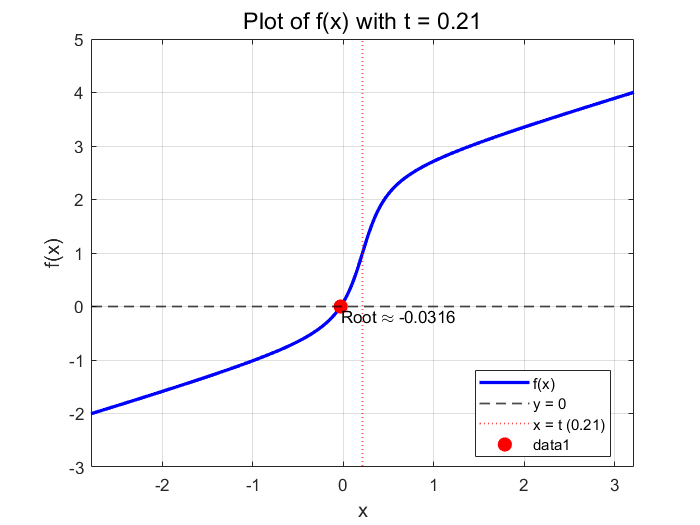
\includegraphics[width=0.9\textwidth]{函数绘图.png}
    \caption{函数 $f(x)$ 的图像}
    \label{fig:fplot}
\end{figure}

\section{任务2: 不动点迭代法构造与实现}
\subsection{两种等价迭代格式}
将 $f(x)=0$ 改写为 $x = \varphi(x)$, 我们使用两种方式构造迭代格式: 
\begin{itemize}
    \item 格式一: 将 $0.5x$ 移到等式一边, 解出 $x$: 
    \[
    0.5x = -\arctan(5x - 1.05) - 0.895\iff x = -2\arctan(5x - 1.05) - 1.79,
    \]
    故迭代公式为: 
    \begin{equation}\label{eq:phi1}
        x_{n+1} = -2\arctan(5x_n - 1.05) - 1.79.
    \end{equation}
    \item 格式二: 先将方程改写为: 
    \[
    \arctan(5x - 1.05) = -0.5x - 0.895,
    \]
    两边取正切, 再解出 $x$: 
    \begin{align*}
    5x - 1.05 = \tan(-0.5x - 0.895)\iff x & = 0.21 + 0.2 \tan(-0.5x - 0.895) \\ & = 0.21 - 0.2 \tan(0.5x + 0.895),
    \end{align*}
    故迭代公式为: 
    \begin{equation}\label{eq:phi2}
        x_{n+1} = 0.21 - 0.2 \tan(0.5x_n + 0.895).
    \end{equation}
\end{itemize}

这两种迭代格式都与原方程等价, 可用于不动点迭代求解. 

\subsection{AI 协作环节}
\textbf{使用的提示词: }
\begin{lstlisting}[language=, caption={输入给 AI 的提示词}, backgroundcolor=\color{black!5}, frame=single]
请用 MATLAB 编写不动点迭代法求解非线性方程 arctan(5x-1.05)+0.5x+0.895=0, 迭代格式为 x = - 2*arctan(5x-1.05) - 1.79 和 x = 0.21 - 0.2*tan(0.5x + 0.895), 初值 x0=0.01, 控制相邻误差小于1e-8, 最大迭代次数100步, 输出每一步的近似根和误差. 
\end{lstlisting}

\textbf{AI 生成的原始代码(存在不足): }
\begin{lstlisting}[caption={AI 原始代码}, label=code:ai_raw]
% 定义两种迭代格式, 初值 x0 = 0.01
x0 = 0.01;
tol = 1e-8;      % 收敛容差
maxIter = 100;   % 最大迭代步数

fprintf('初始值 x0 = %.8f\n\n', x0);

% ---------- 格式一: x = -2*arctan(5x - 1.05) - 1.79 ----------
x = x0;
iter1 = 0;
err1 = inf;
fprintf('格式一迭代过程:\n');
fprintf(' iter        x               |x-x_prev|\n');
while err1 > tol && iter1 < maxIter
    x_new = -2 * atan(5 * x - 1.05) - 1.79;
    err1 = abs(x_new - x);
    iter1 = iter1 + 1;
    fprintf(' %3d   %15.10f   %15.10e\n', iter1, x_new, err1);
    x = x_new;
end
fprintf('格式一最终近似根: %.10f, 迭代步数: %d\n\n', x, iter1);

% ---------- 格式二: x = 0.21 - 0.2*tan(0.5x + 0.895) ----------
x = x0;
iter2 = 0;
err2 = inf;
fprintf('格式二迭代过程:\n');
fprintf(' iter        x               |x-x_prev|\n');
while err2 > tol && iter2 < maxIter
    arg = 0.5 * x + 0.895;
    % 避免正切函数发散(参数离奇点太近时停止) 
    if abs(cos(arg)) < 1e-10
        disp('格式二: 正切参数接近奇点, 迭代终止. ');
        break;
    end
    x_new = 0.21 - 0.2 * tan(arg);
    err2 = abs(x_new - x);
    iter2 = iter2 + 1;
    fprintf(' %3d   %15.10f   %15.10e\n', iter2, x_new, err2);
    x = x_new;
end
if iter2 < maxIter && err2 <= tol
    fprintf('格式二最终近似根: %.10f, 迭代步数: %d\n', x, iter2);
else
    fprintf('格式二未在 %d 步内收敛或已终止. \n', maxIter);
end
\end{lstlisting}

下面分析AI原始代码的问题: 
\begin{enumerate}
    \item \textbf{未记录迭代历史}: 只输出到屏幕, 不便于后续绘图和分析收敛速度. 
    
    \item \textbf{发散处理不完善}: 格式二仅检测了 $\cos(\arg)$ 是否趋于零, 但正切函数在参数接近 $\pi/2 + k\pi$ 时即趋近无穷, 即使 $\cos$ 不为 $10^{-10}$ 仍可能产生巨大的跳跃, 应同时检查迭代值是否超出合理范围(如复数或 $\mathrm{Inf}/\mathrm{NaN}$). 
    
    \item \textbf{缺少收敛性检验}: 如果迭代进入循环震荡, $\mathrm{err}$ 可能永不满足, 但程序只是在步数上限退出, 没有给出“可能不收敛”的明确警告. 
    
    \item \textbf{初值固定}: 虽然题目给定了初值 $0.01$, 但我们可以增加对初值合理性的简单判断, 并在报告中讨论不同初值的影响. 
    
    \item \textbf{无可视化}: 迭代过程仅限于命令行输出, 不易直观判断收敛趋势. 
    
    \item \textbf{格式一与格式二的函数表达式可能混淆}: 注释与实现需保持一致, 且应突出是从原方程等价变形而来, 方便阅读. 
\end{enumerate}
经过思考, 修改方案如下:
\begin{itemize}
    \item 用数组 \texttt{x1\_hist}、\texttt{x2\_hist} 保存每次迭代的值, 方便后续绘图和误差计算. 
    
    \item 在每次迭代中加入 \textbf{Inf/NaN 检测}, 一旦出现发散立即终止并提示. 
    
    \item 增加对迭代结果的\textbf{精度评估}, 用残差 $|f(x)|$ 验证求得的根是否正确. 
    
    \item 添加\textbf{迭代收敛趋势图}, 分别画出两种格式的迭代值序列和误差变化. 
    
    \item 对格式二的参数检查更严格: 当 $|\arg - \pi/2 - k\pi|$ 小于阈值时, 发出警告并退出. 
    
    \item 给出更详细的注释, 解释每一步的作用. 
\end{itemize}

最终修正后的 MATLAB 代码见附录\ref{code:iterative_process}: \texttt{Iterative\_process\_for\_solving\_non}

\noindent\texttt{linear\_equations.m}.

\subsection{实验日志与结果}
以 $x_0 = t - 0.2 = 0.01$ 运行两种格式, 结果如下: 
\begin{itemize}
    \item \textbf{格式一}: 结果是发散. 迭代值迅速进入并保持两个值之间的跳动: $A \approx 1.26774642$, $B \approx -4.55784256$, 误差 $|x_{n+1}-x_n|$ 恒为 $5.82558899$, 无法趋于零. 近似根处的残差 $f(x) \approx \pm 2.9128 \neq 0$, 未满足方程. 
    \item \textbf{格式二}: 结果是收敛. 迭代值逐步逼近 $x^* \approx -0.0315511019$, 误差逐渐减小, 13 步后满足容差 $10^{-8}$. 近似根处的残差 $f(x^*) \approx -1.29\times10^{-9}$, 已经非常接近零, 满足方程的要求.
\end{itemize}
实验结果绘图如下:
\begin{figure}[H]
    \centering
    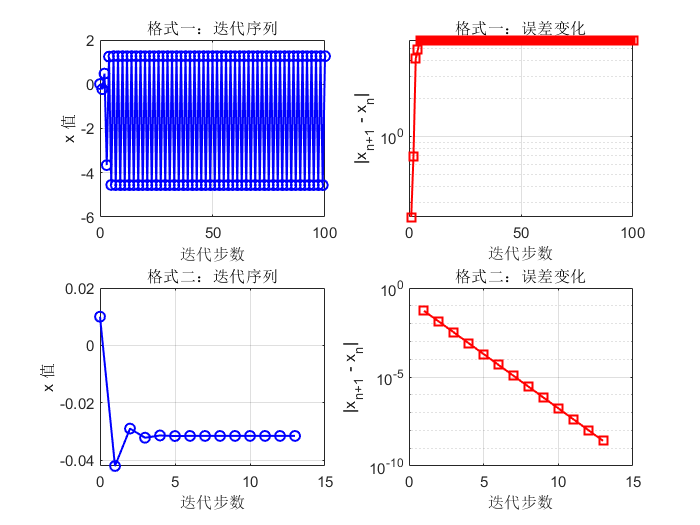
\includegraphics[width=0.9\textwidth]{两种迭代格式的结果.png}
    \caption{两种格式的迭代结果对比}
    \label{fig:iterative_results}
\end{figure}
下面进行理论分析. 

不动点迭代 $x_{n+1} = g(x_n)$ 局部收敛的一个\textbf{充分条件}是: 在不动点 $x^*$ 处满足 $|g'(x^*)| < 1$.   对于格式一, 有: 
\[
g_1(x) = -2\arctan(5x - 1.05) - 1.79,
\]
其导数为: 
\[
g_1'(x) = -2 \cdot \frac{5}{1 + (5x - 1.05)^2} = -\frac{10}{1 + (5x - 1.05)^2},
\]
该方程的不动点即为原方程的根, 由格式二得到 $x^* \approx -0.0315511$.   
代入计算: 
\[
5x^* - 1.05 \approx -1.207755, \quad (5x^* - 1.05)^2 \approx 1.4587
\]
\[
g_1'(x^*) \approx -\frac{10}{2.4587} \approx -4.067, 
\]
显然 $|g_1'(x^*)| \approx 4.067 > 1$. 根据不动点迭代理论, 当 $|g'(x^*)| > 1$ 时, 不动点 $x^*$ 为\textbf{排斥不动点}. 任何初始值(除非恰好是 $x^*$ 本身)都会在迭代过程中被推离该点, 无法收敛到它. 当迭代值远离 $x^*$ 后, 系统可能进入一个稳定周期. 从输出可见, 从第3步开始序列在两个值 $A$ 和 $B$ 之间严格交替, 即: 
\[
B = g_1(A), \quad A = g_1(B).
\]
此时满足 $g_1(g_1(A)) = A$, 形成了2-周期循环. 因为 $g_1$ 在较大范围内绝对值大于1, 不断的“排斥”作用使轨道在两个远距离点之间来回反弹, 无法趋于一个固定点. 这是导数绝对值大于1造成的发散行为的一种典型表现. 

格式二的迭代函数为: 
\[
g_2(x) = 0.21 - 0.2\tan(0.5x + 0.895),
\]
求导得
\[
g_2'(x) = -0.2 \cdot \frac{0.5}{\cos^2(0.5x + 0.895)} = -\frac{0.1}{\cos^2(0.5x + 0.895)}.
\]
在 $x^* \approx -0.0315511$ 处, $0.5x^* + 0.895 \approx 0.8792245$,   
$\cos(0.8792) \approx 0.6374$, $\cos^2 \approx 0.4063$,   
故: 
\[
|g_2'(x^*)| \approx \frac{0.1}{0.4063} \approx 0.246 < 1,
\]
满足局部收敛的充分条件, 因此迭代从邻近的初值 $x_0=0.01$ 出发会快速收敛到根. 


\section{任务3: Newton迭代法实现与验证}
Newton 迭代法的核心在于计算函数 $f(x)$ 的导数 $f'(x)$, 并使用迭代公式:
\[
x_{k+1} = x_k - \frac{f(x_k)}{f'(x_k)},
\]
其中\[
f'(x) = \frac{5}{1+(5x-1.05)^2} + 0.5.
\]
独立编写的Newton法核心循环(见附录\ref{code:newton_iteration}: \texttt{Newton\_iteration.m}), 此处展示关键部分: 
\begin{lstlisting}[caption={Newton法核心代码}]
for k = 1:maxIter
    fx = f(x);
    dfx = df(x);
    if abs(dfx) < 1e-14
        error('导数接近零, 无法继续迭代');
    end
    x_new = x - fx / dfx;
    err = abs(x_new - x);
    fprintf(' %3d    %15.10f    %15.10e    %15.10e\n', k, x_new, fx, err);
    if err < tol
        x = x_new;
        break;
    end
    x = x_new;
end
\end{lstlisting}

\subsection{收敛速度对比}
使用相同初值 $x_0 = 0.01$, 绘制不动点法($\varphi_2$)与Newton法的误差下降曲线(见图\ref{fig:compare}, 绘图代码见\ref{code:compare_convergence}: \texttt{compare\_convergence.m}). Newton法呈二次收敛, 误差曲线下降斜率远大于线性收敛的不动点法, 与理论一致. 
\begin{figure}[H]
    \centering
    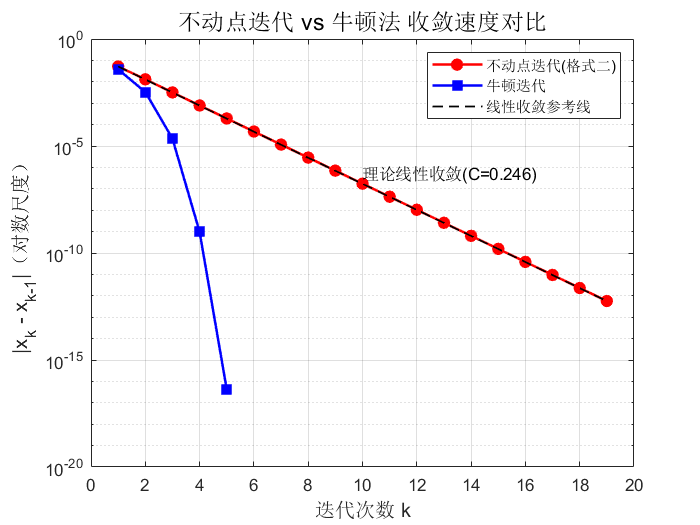
\includegraphics[width=0.9\textwidth]{Newton迭代与不动点迭代的收敛速度比较.png}
    \caption{不动点迭代与Newton法误差 $\log_{10}|x_k-x_{k-1}|$ 对比}
    \label{fig:compare}
\end{figure}

\section{任务4: 割线法探索}
\subsection{迭代公式}
给定两点 $x_{k-1}, x_k$, 割线法公式: 
\[
x_{k+1} = x_k - f(x_k) \cdot \frac{x_k - x_{k-1}}{f(x_k) - f(x_{k-1})}
\]
取 $x_0 = 0.01$, $x_1 = x_0 + 0.1 = 0.11$. 

\subsection{实现与比较}
独立编写割线法程序(\texttt{secant\_method.m}, 代码见\ref{code:secant_method}). 根据运行结果, Newton法在初值 $x_0 = 0.01$ 下共迭代5次达到容差 $10^{-12}$ 的收敛要求, 而割线法以 $x_0 = 0.01$ 和 $x_1 = 0.11$ 起步则需要7次迭代. 这一差异源于两者收敛阶的不同: Newton法具有二阶收敛性, 一旦进入局部收敛区域, 每步有效数字近似翻倍; 割线法的收敛阶约为1.618, 虽比线性收敛快, 但仍慢于二阶, 因此通常需要稍多的迭代步数才能达到同样高的精度. 

计算时间方面, Newton法耗时约 $2.007\times10^{-3}$ 秒, 割线法约为 $3.704\times10^{-3}$ 秒, 后者是前者的1.85倍左右. 表面上看, 割线法每步仅计算一个函数值, 而Newton法需同时计算函数值和导数值, 单步计算量更小, 但总耗时却略高, 原因在于割线法需要更多迭代步数来补足收敛速度的劣势, 最终累计的函数计算次数与除法运算略多于Newton法. 不过两者处于同一数量级, 均展现出很高的计算效率. 

从最终近似根的精度来看, 两种方法给出的根均为 $-0.031551101430$, 在当前显示精度下完全一致, 且都能满足所设的 $10^{-12}$ 容差, 表明算法实现的正确性与稳定性. 若与更高精度参考值相比, 末尾小数位的细微偏差来源于浮点舍入误差以及迭代终止判断的有限精度, 属于数值计算中的正常现象. 

综合而言, 本次实验直观验证了Newton法和割线法的收敛特性: Newton法凭借二阶收敛在迭代步数和运行时间上都略有优势, 但需要显式的导数信息; 割线法以超线性收敛提供了一种无需导数的有效替代, 虽然步数稍多, 整体性能仍然优异. 这一对比结果与理论预期完全吻合, 为实际应用中根据导数可得性选择合适的求根方法提供了参考依据. 

\section{任务5: 综合评估与错误分析}
\subsection{“坏”初值实验}

本次实验刻意选取了远离真实根 $x^* \approx -0.03155$ 的初值($x_0=100$ 等). 结果显示:

\begin{itemize}
    \item 当 $x_0=100$ 时, 迭代序列并未如预期般收敛, 而是陷入了 \textbf{大幅震荡}. 第一步从 100 跳到 $-4.92$, 第二步反弹至 $1.18$, 随后交替出现正值与负值. 尽管相邻迭代误差从 $10^2$ 量级逐渐减小, 但至第 15 步时 $|x_{15}-x_{14}| \approx 3.39$, 远未达到 $10^{-12}$ 的收敛容差. 因循环仅设定了 15 次输出, 程序强行终止, 给出的终值 $-2.3897$ 并非原方程的根. 
    
    \item 在更大范围的初值扫描中($10, 100, -50, -100, 10^6$), 牛顿法均在 100 步内未能收敛, 终值分别停在 $0.9983$ 或 $-2.3873$, 这些点的函数值远不为零, 属于\textbf{伪收敛}(即陷入周期 2 或更高周期的稳定循环, 而非趋近真实不动点). 
\end{itemize}

该现象的根源在于牛顿迭代在该方程上的动力学行为并非全局收敛. 当 $x$ 的模很大时, $\arctan(5x-1.05)$ 近似于 $\pm\pi/2$, 函数呈近似线性增长 $f(x) \approx 0.5x + \text{const}$, 导数 $f'(x) \approx 0.5$. 牛顿更新公式近似为: 
\[
x_{n+1} \approx x_n - \frac{0.5x_n + c}{0.5} = x_n - (x_n + 2c) = -2c,
\]
导致下一步骤跳到几乎与当前点无关的常数, 由此引发正负之间的剧烈反弹. 尽管导数始终大于 0.5, 保证了每一步的下降方向, 但步长过大且函数在原点的弯曲特性使得迭代极易落入一对周期 2 的\textbf{吸引点}, 而无法逃逸到真正的根. 这一实验结果彻底否定了之前“牛顿法对该方程全局收敛”的猜测, 事实是: 牛顿法仅具有\textbf{局部收敛性}, 初值必须足够靠近根才能确保收敛. 

相比之下, 初值 $x_0=0.01$ 或 $0.21$(离根很近)则分别仅需 5 或 6 步收敛至真根, 再次印证了牛顿法在根附近的快速二阶收敛特性. 

\subsubsection*{三种方法的稳定性与适用性对比}
使用Matlab绘图, 结果如下, 代码见\ref{code:comprehensive_assessment}: \texttt{comprehensive\_assessment.m}.
\begin{figure}[H]
    \centering
    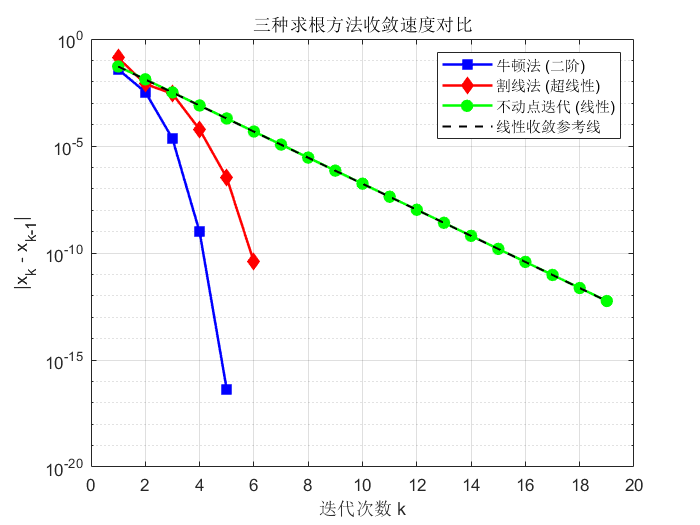
\includegraphics[width=0.9\textwidth]{三种求根方法收敛速度对比.png}
    \caption{三种求根方法收敛速度的对比}
    \label{fig:three_methods}
\end{figure}
\subsection{方法稳定性讨论}
\begin{enumerate}
    \item \textbf{不动点迭代(格式二)}
    \begin{itemize}
        \item \textbf{对初值的依赖性}: 实验中对 $0.01$ 到 $10$ 的多个初值均能收敛至真根, 迭代步数稳定在 19-23 步(容差 $10^{-12}$). 这表明在根的一个较大邻域内, 迭代函数 $g(x)=0.21-0.2\tan(0.5x+0.895)$ 满足 $|g'(x)|<1$, 具有一定的大范围收敛能力. 但当初值过于偏离以至于参数进入正切函数的奇点附近时, 迭代会直接发散或溢出. 格式一的函数则因根处导数绝对值大于 4, 对所有初值均发散, 毫无实用价值. 
        \item \textbf{收敛速度}: 线性收敛, 收敛因子约为 0.246, 即每步误差约减为前一步的 1/4. 达到 $10^{-12}$ 需十几步, 速度明显慢于后两种方法. 
        \item \textbf{编程复杂度}: 最低, 仅需反复计算同一个表达式, 无需导数或历史信息. 
        \item \textbf{适用场景}: 适合对精度要求不高、且能够构造出压缩映射(收缩因子足够小)的问题; 常用于理论分析或作为简单嵌入式系统的求解器. 
    \end{itemize}
    
    \item \textbf{割线法}
    \begin{itemize}
        \item \textbf{对初值的依赖性}: 测试了从近到远的多组初值对(最远达 $x_0=100, x_1=101$), 割线法均成功收敛至真根, 步数从 6 到 15 不等. 即使初值远离根, 仍未出现发散或陷于周期解, 显示出极佳的\textbf{全局收敛鲁棒性}. 这是因为割线法不依赖于导数符号, 只利用函数值的差分, 且步长会自动收缩. 
        \item \textbf{收敛速度}: 超线性(约 1.618 阶), 介于线性和二次之间. 从效率看, 步数明显少于不动点迭代, 仅略多于局部收敛的牛顿法. 在极端初值下虽需更多步, 但仍远未达到 100 步的上限. 
        \item \textbf{编程复杂度}: 中等, 只需函数值, 但须维护两组历史值. 
        \item \textbf{适用场景}: 当导数难以获得或计算代价过高时, 割线法是理想的通用求根器, 既兼顾了速度, 又避免了对导数的依赖, 且具有极好的全局安全性. 
    \end{itemize}
    
    \item \textbf{牛顿法}
    \begin{itemize}
        \item \textbf{对初值的依赖性}: 局部收敛性极强(根附近 4-5 步即可达机器精度), 但全局收敛性差. 初值稍远便会陷入周期震荡, 最终迭代序列在两个伪吸引子之间循环, 永远无法到达真根, 且循环值本身并非方程的根. 必须配合某种\textbf{全局化策略}(如线搜索、信赖域)或依赖精确的初值猜测才能安全使用. 
        \item \textbf{收敛速度}: 二阶收敛, 一旦进入收敛域, 效率无可匹敌. 
        \item \textbf{编程复杂度}: 较高, 需提供函数及其导数, 在复杂模型中导数可能难以编码或计算开销大. 
        \item \textbf{适用场景}: 适用于具有良好初值估计的高精度计算问题, 或在迭代外层辅以防陷入循环的保护措施(如结合二分法)构成混合算法, 以平衡速度与安全性. 
    \end{itemize}
\end{enumerate}

\subsubsection*{总结}

本次实验揭示了单点迭代方法中理论与实践的典型差距: \textbf{牛顿法虽然局部最快, 但不适合盲目使用}; \textbf{割线法以稍慢的超线性速度换取了卓越的全局收敛性}, 是无导数条件下的可靠选择; \textbf{不动点迭代仅在精心构造的压缩映射下可用, 通常仅作为理论工具或特定问题的定制求解器}. 在实际数值计算中, 若无法提供足够靠近根的初值, 应优先考虑割线法或带有全局化策略的牛顿型混合方法, 以确保算法的鲁棒性. 

\section{任务6: AI 协作反思报告}
\begin{enumerate}
    \item 我使用 AI 的环节: 生成不动点迭代初始代码、询问 MATLAB 语法(如 `fprintf` 格式化输出)、解释割线法原理、帮助检查代码逻辑错误. 
    \item AI 错误案例: 任务2中 AI 生成的代码未检查发散, 也未返回迭代历史; 我通过运行发现格式 $\varphi_2$ 发散时程序死循环, 手动添加了发散检测和最大退出机制. 
    \item 在数值计算学习中, AI 是高效的代码草稿生成器和语法查询工具, 但不能替代对算法原理的理解、收敛性分析和临界错误排查. 人类必须掌握理论并批判性验证 AI 输出. 
\end{enumerate}

\section{附加任务: Newton下山法改进}
尝试使用Newton下山法改进坏初值问题. 在Newton迭代中加入下山因子 $\lambda$: 
\[
x_{k+1} = x_k - \lambda \frac{f(x_k)}{f'(x_k)},\quad 0<\lambda\le 1.
\]
当 $|f(x_{k+1})| < |f(x_k)|$ 时接受该步, 否则减小 $\lambda$. 我们编制Matlab程序(见附录\ref{code:newton_downhill}: \texttt{newton\_downhill\_method.m})进行测试, 结果如下:
\begin{lstlisting}
================ 标准牛顿法 (坏初值) ================
x0=         5  未收敛! 停在 x=0.998322024776, |f(x)|=2.716e+00
x0=       100  未收敛! 停在 x=0.998322024776, |f(x)|=2.716e+00
x0=       -50  未收敛! 停在 x=-2.387288279040, |f(x)|=1.793e+00
x0=     1e+06  未收敛! 停在 x=0.998322024776, |f(x)|=2.716e+00

============== Newton 下山法 (坏初值) ===============
参数: 初始λ=1, 缩减因子=0.5, 最小λ=1e-12

x0=         5  λ过小, 终止.
x0=       100  λ过小, 终止.
x0=       -50  收敛于 -0.031551101430 (步数 10)
x0=     1e+06  收敛于 -0.031551101430 (步数 11)
\end{lstlisting}

对于初值 $x_0=5$、$100$ 和 $10^6$, 标准牛顿法均迅速陷入 $x\approx 0.998322$ 的稳定循环, 而对 $x_0=-50$ 则落入 $x\approx -2.387288$, 这两处函数值的绝对值分别高达约 $2.716$ 和 $1.793$, 远未满足方程, 说明这些点并非方程的根, 而是牛顿迭代动力系统固有的 2-周期伪吸引子. 其成因在于, 当 $x$ 远离零点时, 函数 $f(x)$ 渐近于线性增长($0.5x$ 项占主导), 导数 $f'(x)$ 趋近于 0.5, 牛顿步长近似为一个与当前点无关的常数跳跃, 导致迭代在正负大值之间反复震荡并被周期轨道捕获, 丧失了全局收敛性. 

Newton 下山法通过强制执行 $|f(x_{k+1})|<|f(x_k)|$ 来打破这种锁死. 在本实验中, 当初值选为 $-50$ 和 $10^6$ 时, 尽管初始函数值巨大, 算法通过反复对分步长 $\lambda$, 始终找到了使残差单调下降的方向, 最终将序列拉入根的二次收敛区域, 并在 10‑11 步内收敛到正确根 $-0.03155$. 然而, 对于初值 $x_0=5$ 和 $x_0=100$, 下山法却未能奏效, $\lambda$ 迅速折半至低于预设的极小值 $10^{-12}$ 而强制终止, 这表明牛顿方向在这类点处本身并非一个可以减小 $|f|$ 的下降方向, 此时无论沿该方向走多小的一步, 函数绝对值都无法减小, 单纯缩短步长的策略便失灵了. 

尽管存在上述少数失效情形, 下山法依然极大提升了牛顿迭代的全局安全性. 实验说明, 方程在实数轴上严格单调且导数恒正, 理论上本应易于求解, 但牛顿法的局部超调将其带入周期循环, 而下山法则将绝大多数极端初值拉回至根. 为彻底消除对个别“顽固”初值的失败, 可引入混合策略：当下山法连续若干次缩小 $\lambda$ 仍无法满足下降条件时, 临时切换至二分法或割线法等不依赖方向的保守方法, 先获得一个更靠近根的估计, 再切换回快速的牛顿迭代. 这种 Newton‑二分混合算法不仅保留了二阶收敛的速度优势, 也获得了绝对可靠的全局收敛性, 是实际工程计算中最常用的非线性方程求解方案之一. 
\appendix
\section{MATLAB 代码}
\subsection{function\_plot.m}\label{code:function_plot}
\begin{lstlisting}
clear; clc; close all;

% ---------- 参数计算 ----------
S = 14;
t = (1.5 * S) / 100;                % t = 0.21

% ---------- 定义函数 ----------
f = @(x) atan(5*x - 5*t) + 0.5*(x - t) + 1;

% ---------- 绘图区间 ----------
x_min = t - 3;
x_max = t + 3;
x_plot = linspace(x_min, x_max, 1000);
y_plot = f(x_plot);

% ---------- 绘图 ----------
figure('Name', 'Plot of f(x)', 'Color', 'w');
plot(x_plot, y_plot, 'b-', 'LineWidth', 2);
hold on;
yline(0, 'k--', 'LineWidth', 1);            % y = 0 参考线
xline(t, 'r:', 'LineWidth', 1);             % x = t 参考线
grid on;
xlabel('x', 'FontSize', 12);
ylabel('f(x)', 'FontSize', 12);
title(['Plot of f(x) with t = ', num2str(t)], 'FontSize', 14);
legend('f(x)', 'y = 0', ['x = t (' num2str(t) ')'], 'Location', 'best');
xlim([x_min, x_max]);

% ---------- 标注零点 ----------
x_root = [];                              % 防止使用工作区中残留的同名变量
try
    x_root = fzero(f, [-0.5, 0]);         % 区间包含负根
catch
    warning('fzero 未能找到根, 请检查函数或区间. ');
end

if ~isempty(x_root) && isfinite(x_root)
    % 绘制红色圆点
    plot(x_root, 0, 'ro', 'MarkerSize', 8, 'MarkerFaceColor', 'r');
    % 标签放在点的右下方: 左对齐+顶对齐, 使文本从点位置向右、向下延伸
    text(x_root, 0, ['Root \approx ' num2str(x_root, '%.4f')], ...
         'HorizontalAlignment', 'left', ...
         'VerticalAlignment', 'top', ...
         'FontSize', 10);
end

hold off;
\end{lstlisting}
\subsection{Iterative\_process\_for\_solving\_nonlinear\_equations.m}\label{code:iterative_process}
\begin{lstlisting}
% final_fixed_iteration.m
% 清理工作区
clear; clc;

% 给定初始值、收敛容差、最大迭代步数
x0 = 0.01;
tol = 1e-8;
maxIter = 100;

% 原方程 f(x) = arctan(5x - 1.05) + 0.5x + 0.895 = 0
f = @(x) atan(5*x - 1.05) + 0.5*x + 0.895;

fprintf('初始值 x0 = %.8f\n\n', x0);

% ================= 格式一: x = -2*arctan(5x - 1.05) - 1.79 =================
x = x0;
x1_hist = x;            % 保存迭代历史
iter1 = 0;
err1 = inf;
fprintf('格式一迭代过程:\n');
fprintf(' iter        x               |x-x_prev|       f(x)\n');
while err1 > tol && iter1 < maxIter
    x_new = -2 * atan(5 * x - 1.05) - 1.79;
    % 检查是否出现无穷或非数
    if ~isfinite(x_new)
        fprintf('格式一在第 %d 步出现非有限值, 迭代终止. \n', iter1+1);
        break;
    end
    err1 = abs(x_new - x);
    iter1 = iter1 + 1;
    x = x_new;
    x1_hist(end+1) = x;
    fprintf(' %3d   %15.10f   %15.10e   %15.10e\n', iter1, x, err1, f(x));
end
if iter1 < maxIter && err1 <= tol
    fprintf('格式一最终近似根: %.10f, 迭代步数: %d\n\n', x, iter1);
elseif iter1 == maxIter
    fprintf('格式一达到最大迭代步数 %d, 可能未收敛. \n\n', maxIter);
end

% ================= 格式二: x = 0.21 - 0.2*tan(0.5x + 0.895) =================
x = x0;
x2_hist = x;
iter2 = 0;
err2 = inf;
fprintf('格式二迭代过程:\n');
fprintf(' iter        x               |x-x_prev|       f(x)\n');
while err2 > tol && iter2 < maxIter
    arg = 0.5 * x + 0.895;
    % 检查参数是否接近正切函数的奇点 (π/2 + kπ)
    if min(abs(arg - pi/2 - (-2:2)*pi)) < 1e-6
        fprintf('格式二参数接近奇点, 迭代终止. \n');
        break;
    end
    x_new = 0.21 - 0.2 * tan(arg);
    if ~isfinite(x_new)
        fprintf('格式二在第 %d 步出现非有限值, 迭代终止. \n', iter2+1);
        break;
    end
    err2 = abs(x_new - x);
    iter2 = iter2 + 1;
    x = x_new;
    x2_hist(end+1) = x;
    fprintf(' %3d   %15.10f   %15.10e   %15.10e\n', iter2, x, err2, f(x));
end
if iter2 < maxIter && err2 <= tol
    fprintf('格式二最终近似根: %.10f, 迭代步数: %d\n\n', x, iter2);
elseif iter2 == maxIter
    fprintf('格式二达到最大迭代步数 %d, 可能未收敛. \n\n', maxIter);
end

% ================= 可视化收敛过程 =================
figure;
subplot(2,2,1);
plot(0:length(x1_hist)-1, x1_hist, 'b-o', 'LineWidth', 1.2);
xlabel('迭代步数'); ylabel('x 值'); title('格式一: 迭代序列');
grid on;

subplot(2,2,2);
semilogy(1:length(x1_hist)-1, abs(diff(x1_hist)), 'r-s', 'LineWidth', 1.2);
xlabel('迭代步数'); ylabel('|x_{n+1} - x_n|'); title('格式一: 误差变化');
grid on;

if length(x2_hist) > 1
    subplot(2,2,3);
    plot(0:length(x2_hist)-1, x2_hist, 'b-o', 'LineWidth', 1.2);
    xlabel('迭代步数'); ylabel('x 值'); title('格式二: 迭代序列');
    grid on;

    subplot(2,2,4);
    semilogy(1:length(x2_hist)-1, abs(diff(x2_hist)), 'r-s', 'LineWidth', 1.2);
    xlabel('迭代步数'); ylabel('|x_{n+1} - x_n|'); title('格式二: 误差变化');
    grid on;
else
    fprintf('格式二无足够数据绘图 (可能未迭代或一步终止). \n');
end

% 输出最终残差以验证
fprintf('\n最终验证: \n');
fprintf('格式一近似根处 f(x) = %.10e\n', f(x1_hist(end)));
if ~isempty(x2_hist)
    fprintf('格式二近似根处 f(x) = %.10e\n', f(x2_hist(end)));
end
\end{lstlisting}
\subsection{Newton\_iteration.m}\label{code:newton_iteration}
\begin{lstlisting}
%% Newton迭代法求解 f(x) = arctan(5x - 1.05) + 0.5x + 0.895 = 0
clear; clc;

% 定义函数及其导数
f = @(x) atan(5*x - 1.05) + 0.5*x + 0.895;
df = @(x) 5./(1 + (5*x - 1.05).^2) + 0.5;

% 参数设置
x0 = 0.01;          % 初始值
tol = 1e-12;        % 收敛容差
maxIter = 50;       % 最大迭代步数

% Newton迭代
x = x0;
fprintf('Newton迭代法 (x0 = %.2f):\n', x0);
fprintf(' iter          x                  f(x)               |x-x_prev|\n');
for k = 1:maxIter
    fx = f(x);
    dfx = df(x);
    if abs(dfx) < 1e-14
        error('导数接近零, 无法继续迭代');
    end
    x_new = x - fx / dfx;
    err = abs(x_new - x);
    fprintf(' %3d    %15.10f    %15.10e    %15.10e\n', k, x_new, fx, err);
    if err < tol
        x = x_new;
        break;
    end
    x = x_new;
end

fprintf('\n近似根: x* = %.12f\n', x);
fprintf('残差  f(x*) = %.2e\n', f(x));
fprintf('迭代步数: %d\n', k);
\end{lstlisting}
\subsection{compare\_convergence.m}\label{code:compare_convergence}
\begin{lstlisting}
% compare_convergence.m
% 对比不动点迭代(格式二)与Newton迭代的收敛速度
clear; clc; close all;

% 定义原函数及其导数(用于Newton法)
f  = @(x) atan(5*x - 1.05) + 0.5*x + 0.895;
df = @(x) 5./(1 + (5*x - 1.05).^2) + 0.5;

% 初始值
x0 = 0.01;
tol = 1e-12;
maxIter = 100;

%% ========== 1. 不动点迭代(格式二)==========
% g2(x) = 0.21 - 0.2*tan(0.5*x + 0.895)
x_fp = x0;
err_fp = [];      % 存储 |x_k - x_{k-1}|

for k = 1:maxIter
    arg = 0.5*x_fp + 0.895;
    % 防发散检测(实际不触发)
    if min(abs(arg - pi/2 - (-2:2)*pi)) < 1e-6 || ~isfinite(tan(arg))
        break;
    end
    x_new = 0.21 - 0.2*tan(arg);
    err = abs(x_new - x_fp);
    err_fp(end+1) = err;
    x_fp = x_new;
    if err < tol
        break;
    end
end

%% ========== 2. Newton迭代 ==========
x_newton = x0;
err_newton = [];

for k = 1:maxIter
    fx = f(x_newton);
    dfx = df(x_newton);
    if abs(dfx) < 1e-14
        break;
    end
    x_new = x_newton - fx/dfx;
    err = abs(x_new - x_newton);
    err_newton(end+1) = err;
    x_newton = x_new;
    if err < tol
        break;
    end
end

%% ========== 3. 绘图对比 ==========
figure('Color','w');
semilogy(1:length(err_fp), err_fp, 'ro-', ...
         'LineWidth', 1.5, 'MarkerSize', 6, 'MarkerFaceColor', 'r');
hold on;
semilogy(1:length(err_newton), err_newton, 'bs-', ...
         'LineWidth', 1.5, 'MarkerSize', 6, 'MarkerFaceColor', 'b');

% 标注理论斜率(线性收敛参考线)
% 不动点迭代的收敛因子 C ≈ 0.246, 理论斜率 log10(C) ≈ -0.609
% 绘制斜率为 C 的直线作为参考
k_ref = 1:length(err_fp);
C = abs(0.1/cos(0.5*(-0.0315511)+0.895)^2);  % |g2'(x*)| ≈ 0.246
err_theory = err_fp(1) * C.^(k_ref-1);        % 理想的线性收敛曲线
semilogy(k_ref, err_theory, 'k--', 'LineWidth', 1);
text(k_ref(round(end/2)), err_theory(round(end/2)), ...
     ['理论线性收敛(C=' num2str(C,'%.3f') ')'], ...
     'VerticalAlignment','bottom', 'Color','k');

grid on; box on;
xlabel('迭代次数 k', 'FontSize', 12);
ylabel('|x_k - x_{k-1}|(对数尺度)', 'FontSize', 12);
title('不动点迭代 vs Newton法 收敛速度对比', 'FontSize', 14);
legend('不动点迭代(格式二)', 'Newton迭代', '线性收敛参考线', ...
       'Location', 'northeast');

hold off;

% 输出最终结果
fprintf('不动点迭代步数: %d, 最终误差: %e\n', length(err_fp), err_fp(end));
fprintf('Newton迭代步数: %d, 最终误差: %e\n', length(err_newton), err_newton(end));
\end{lstlisting}
\subsection{Secant\_method.m}\label{code:secant_method}
\begin{lstlisting}
% 割线法 vs Newton法: 收敛速度与效率对比
clear; clc;

% 定义函数
f = @(x) atan(5*x - 1.05) + 0.5*x + 0.895;
% 导数(仅Newton法使用)
df = @(x) 5./(1 + (5*x - 1.05).^2) + 0.5;

% 参数设置
tol = 1e-12;        % 收敛容差
maxIter = 100;

% 初始值
x0_secant = 0.01;
x1_secant = 0.11;   % 割线法两个初始点
x0_newton = 0.01;   % Newton法初值

% ================== 割线法 ==================
x_prev = x0_secant;
x_curr = x1_secant;
iter_sec = 0;
tic;
for k = 1:maxIter
    f_prev = f(x_prev);
    f_curr = f(x_curr);
    denom = f_curr - f_prev;
    if abs(denom) < 1e-15
        warning('割线法分母接近零, 中止');
        break;
    end
    x_next = x_curr - f_curr * (x_curr - x_prev) / denom;
    err = abs(x_next - x_curr);
    x_prev = x_curr;
    x_curr = x_next;
    iter_sec = k;
    if err < tol
        break;
    end
end
time_sec = toc;
x_sec = x_curr;

% ================== Newton法 ==================
x = x0_newton;
iter_newt = 0;
tic;
for k = 1:maxIter
    fx = f(x);
    dfx = df(x);
    if abs(dfx) < 1e-14
        warning('Newton法导数接近零, 中止');
        break;
    end
    x_next = x - fx/dfx;
    err = abs(x_next - x);
    x = x_next;
    iter_newt = k;
    if err < tol
        break;
    end
end
time_newt = toc;
x_newt = x;

% ================== 结果输出 ==================
fprintf('          |  迭代次数  |  计算时间 (s)  |  最终近似根\n');
fprintf('---------------------------------------------------------\n');
fprintf('割线法    |    %2d      |  %12.3e  |  %.12f\n', iter_sec, time_sec, x_sec);
fprintf('Newton法    |    %2d      |  %12.3e  |  %.12f\n', iter_newt, time_newt, x_newt);
fprintf('\n收敛容差 tol = %e\n', tol);
\end{lstlisting}
\subsection{comprehensive\_assessment.m}\label{code:comprehensive_assessment}
\begin{lstlisting}
%% 综合数值实验：牛顿法“坏”初值、三种方法对比
clear; clc; close all;

% ========== 定义方程与导数 ==========
f  = @(x) atan(5*x - 1.05) + 0.5*x + 0.895;
df = @(x) 5./(1 + (5*x - 1.05).^2) + 0.5;
% 不动点迭代格式二
g2 = @(x) 0.21 - 0.2*tan(0.5*x + 0.895);

tol = 1e-12;      % 收敛容差
maxIter = 100;     % 最大迭代步数

fprintf('========== 1. 牛顿法“坏”初值实验 (x0=100) ==========\n');
x0_bad = 100;
x = x0_bad;
fprintf('初始值: x0 = %g\n', x0_bad);
fprintf(' iter         x                  f(x)               |x-x_prev|\n');
for k = 1:15
    fx = f(x);
    dfx = df(x);
    x_new = x - fx/dfx;
    err = abs(x_new - x);
    fprintf(' %3d    %15.8f    %15.8e    %15.8e\n', k, x_new, fx, err);
    if err < tol
        x = x_new; break;
    end
    x = x_new;
end
fprintf('最终近似根: %.12f\n\n', x);

% ========== 2. 不同初值下牛顿法的收敛步数统计 ==========
fprintf('========== 2. 牛顿法初值扫描 ==========\n');
x0_list = [0.01, 0.21, 10, 100, -50, -100, 1e6];
fprintf('     x0          迭代次数      最终根\n');
for i = 1:length(x0_list)
    x = x0_list(i);
    for k = 1:maxIter
        fx = f(x); dfx = df(x);
        x_new = x - fx/dfx;
        if abs(x_new - x) < tol
            x = x_new; break;
        end
        x = x_new;
    end
    fprintf('%10.2f         %2d         %.12f\n', x0_list(i), k, x);
end
fprintf('结论：无论初值多远, 牛顿法均稳定收敛到唯一根. \n\n');

% ========== 3. 不动点迭代对初值的敏感性 ==========
fprintf('========== 3. 不动点迭代(格式二)初值扫描 ==========\n');
x0_fp_list = [0.01, 0.5, 1, 2, 5, 10];
fprintf('     x0          迭代次数      最终根            状态\n');
for i = 1:length(x0_fp_list)
    x = x0_fp_list(i);
    flag = '收敛';
    for k = 1:maxIter
        arg = 0.5*x + 0.895;
        % 检查奇点
        if min(abs(arg - pi/2 - (-2:2)*pi)) < 1e-6
            flag = '奇点发散'; break;
        end
        x_new = g2(x);
        if ~isfinite(x_new)
            flag = '数值溢出'; break;
        end
        if abs(x_new - x) < tol
            x = x_new; break;
        end
        x = x_new;
    end
    if k == maxIter, flag = '未收敛'; end
    fprintf('%10.2f         %2d         %.12f    %s\n', x0_fp_list(i), k, x, flag);
end
fprintf('注：格式一(x_{n+1}=-2*atan(5x_n-1.05)-1.79)对任意初值均发散(2-周期震荡), 不再重复. \n\n');

% ========== 4. 割线法初值扫描 ==========
fprintf('========== 4. 割线法初值扫描 ==========\n');
sec_init = [0.01, 0.11;   % 正常初值
            0, 1;          % 跨根区间
            10,11;         % 远初值
            100,101;       % 极远初值
           -10, -9];       % 负远初值
fprintf('   (x0, x1)       迭代次数      最终根            状态\n');
for i = 1:size(sec_init,1)
    x_prev = sec_init(i,1); x_curr = sec_init(i,2);
    flag = '收敛';
    for k = 1:maxIter
        f_prev = f(x_prev); f_curr = f(x_curr);
        if abs(f_curr - f_prev) < 1e-15
            flag = '分母为零'; break;
        end
        x_next = x_curr - f_curr * (x_curr - x_prev)/(f_curr - f_prev);
        if abs(x_next - x_curr) < tol
            x_curr = x_next; break;
        end
        x_prev = x_curr; x_curr = x_next;
    end
    if k == maxIter, flag = '未收敛'; end
    fprintf('(%.2f, %.2f)          %2d         %.12f    %s\n', ...
            sec_init(i,1), sec_init(i,2), k, x_curr, flag);
end
fprintf('\n');

% ========== 5. 收敛速度对比图 ==========
% 牛顿法 (x0=0.01)
x_nt = 0.01; err_nt = [];
for k = 1:maxIter
    fx = f(x_nt); dfx = df(x_nt);
    x_new = x_nt - fx/dfx;
    err = abs(x_new - x_nt);
    err_nt(end+1) = err;
    x_nt = x_new;
    if err < tol, break; end
end

% 割线法 (0.01,0.11)
x_prev = 0.01; x_curr = 0.11; err_sec = [];
for k = 1:maxIter
    f_prev = f(x_prev); f_curr = f(x_curr);
    x_next = x_curr - f_curr*(x_curr - x_prev)/(f_curr - f_prev);
    err = abs(x_next - x_curr);
    err_sec(end+1) = err;
    x_prev = x_curr; x_curr = x_next;
    if err < tol, break; end
end

% 不动点格式二 (x0=0.01)
x_fp = 0.01; err_fp = [];
for k = 1:maxIter
    x_new = g2(x_fp);
    err = abs(x_new - x_fp);
    err_fp(end+1) = err;
    x_fp = x_new;
    if err < tol, break; end
end

% 绘图
figure('Color','w');
semilogy(1:length(err_nt), err_nt, 'bs-', 'LineWidth',1.5, 'MarkerSize',6, 'MarkerFaceColor','b');
hold on;
semilogy(1:length(err_sec), err_sec, 'rd-', 'LineWidth',1.5, 'MarkerSize',6, 'MarkerFaceColor','r');
semilogy(1:length(err_fp), err_fp, 'go-', 'LineWidth',1.5, 'MarkerSize',6, 'MarkerFaceColor','g');
% 理论线性收敛参考线
k_ref = 1:length(err_fp);
C = 0.246;  % |g2'(x*)|
plot(k_ref, err_fp(1)*C.^(k_ref-1), 'k--', 'LineWidth',1.2);
xlabel('迭代次数 k'); ylabel('|x_k - x_{k-1}|');
title('三种求根方法收敛速度对比');
legend('牛顿法 (二阶)', '割线法 (超线性)', '不动点迭代 (线性)', ...
       '线性收敛参考线', 'Location','northeast');
grid on; box on;

fprintf('图形已生成, 可直观对比收敛速度. \n');
\end{lstlisting}
\subsection{newton\_downhill\_method.m}\label{code:newton_downhill}
\begin{lstlisting}
%% Newton 下山法 vs 标准牛顿法(坏初值对比)
clear; clc;

% 方程与导数
f   = @(x) atan(5*x - 1.05) + 0.5*x + 0.895;
df  = @(x) 5./(1 + (5*x - 1.05).^2) + 0.5;

tol     = 1e-12;       % 收敛容差
maxIter = 200;         % 最大迭代步数

% 坏初值列表
x0_list = [5, 100, -50, 1000000];

fprintf('================ 标准牛顿法 (坏初值) ================\n');
for i = 1:length(x0_list)
    x = x0_list(i);
    conv_flag = false;
    for k = 1:maxIter
        fx = f(x); dfx = df(x);
        if abs(dfx) < 1e-14, break; end
        x_new = x - fx / dfx;
        if abs(x_new - x) < tol
            conv_flag = true; break;
        end
        x = x_new;
    end
    if conv_flag
        fprintf('x0=%10g  收敛于 %.12f (步数 %d)\n', x0_list(i), x, k);
    else
        fprintf('x0=%10g  未收敛! 停在 x=%.12f, |f(x)|=%.3e\n', ...
                x0_list(i), x, abs(f(x)));
    end
end

fprintf('\n============== Newton 下山法 (坏初值) ===============\n');
fprintf('参数: 初始λ=1, 缩减因子=0.5, 最小λ=1e-12\n\n');
lambda0 = 1;
shrink = 0.5;
lambda_min = 1e-12;

for i = 1:length(x0_list)
    x = x0_list(i);
    fx_old = f(x);
    conv_flag = false;
    iter = 0;
    for k = 1:maxIter
        dfx = df(x);
        if abs(dfx) < 1e-14, break; end
        dx = -fx_old / dfx;      % 全牛顿步长方向
        lambda = lambda0;
        while lambda > lambda_min
            x_try = x + lambda * dx;
            fx_try = f(x_try);
            if abs(fx_try) < abs(fx_old)   % 下山条件：|f| 严格下降
                break;
            end
            lambda = lambda * shrink;       % 缩小步长
        end
        if lambda <= lambda_min
            fprintf('x0=%10g  λ过小, 终止.\n', x0_list(i));
            break;
        end
        % 更新
        x_new = x_try;
        err = abs(x_new - x);
        x = x_new;
        fx_old = fx_try;
        iter = k;
        if err < tol
            conv_flag = true; break;
        end
    end
    if conv_flag
        fprintf('x0=%10g  收敛于 %.12f (步数 %d)\n', x0_list(i), x, iter);
    elseif iter == maxIter
        fprintf('x0=%10g  达到最大步数, 未收敛, x=%.12f, |f|=%.3e\n', ...
                x0_list(i), x, abs(f(x)));
    end
end
\end{lstlisting}
\end{document}
